\section{Managing Trust}
\label{sec:mitigation}

The current trust situation inherent in using many cloud --
i.e. trusting many third parties with a wide range of capabilities and
only moderate disincentivizes to violating user trust -- is far from
ideal. This state places private user data and metadata at a high
degree of risk for unapproved exposure or manipulation. It is natural
to ask what solutions might aid in better controlling third party
trust arraignments, reducing this degree of risk involved when
leveraging third party services. While there are a myriad of potential
solutions in this space, ranging form technical to policy, I suggest a
few high level approaches to managing third party trust in this
section.

The trust model presented in \S~\ref{sec:model} discusses to
components of third party trust: the capabilities we entrust to third
parties and the manners in which this trust might be violated. Further
control of third party trust can be exerted to either or both of these
axis. By reducing the degree or trust -- i.e. limiting the number of
capabilities third parties are granted -- users can limit the amount
of harm a third party can inflict should this trust be violated. By
disincentivizing the various types of trust violations, a user can
decreased the likelihood that a third party violated there trust at
all. I'll focus on strategies for each of these goals below.

\subsection{Limiting Capabilities}
\label{sec:mitigation:capabilites}

Limiting the number of capabilities granted to third parties is an
obvious way to reduce the risk of third party trust
violations. Furthermore, controlling which capabilities to trust to a
third party is largely within the control of each individual user,
making this a relatively direct manner in which to reduce the risk of
third party trust violations. In the most extreme case, users can
simply elect to avoid using many third party services, effectively
granting such third parties no capabilities over the data. For most
users, however, such an approach is at best impractical, and in some
cases, simply not possible. Therein lies the crux of third party
capability reduction -- simply reducing capabilities is not
enough. Instead, users must have a way to both reduce capabilities
while also maintaining the ability to benefit from third party
services in the manners to which theory are accustomed. Thus, the true
aim of third party trust reduction is to identify ``trust scruples''
-- situations where third parties are being trusted with more
capabilities than Si strictly necessary to provide the benefits the
user devices from the service. Finding and eliminating such surpluses
allows users to reduce the degree by which they must trust third
parties while also continuing to leverage third party services to
provide desirable benefits.

Fortunately (at least from the perspective of users hoping to find
ways to reduce the amount they must trust third parties), trust
surpluses appear to be relatively common in modern third party
services. Take, for example, the Dropbox file syncing service. As
discussed in \S~\ref{sec:analysis:capabilites}, user currently trust
Dropbox with all available capabilities: storage (\emph{S}), access
(\emph{R}), modification (\emph{W}), and metadata (\emph{M}). In order
to provide Dropbox's core service, however, user really need only
trust Dropbox with a single capability: storage. Thus, granting
Dropbox the access, modification, and metadata capabilities represent
a trust surplus that can conceivably be eliminated without reducing
Dropbox's ability to provide the syncing and sharing benefits users
expect.\footnote{The techniques discussed herein focus primarily on
  limiting surplus access and manipulation capabilities. Unfortunately,
  limiting the metadata capability is historically much more difficult
  than limiting data-related capabilities such as storage, access, or
  manipulation. Thus, until better solutions present themselves, it
  may be necessary to continue granting third party service providers
  the metadata capability -- even in surplus.}

The question then becomes how best to limit Dropbox's access to these
surplus capabilities. As mentioned previously, client-side
cryptographic techniques provide tools for liming the access
capability (e.g. encryption) as well as the modification capability
(e.g. authentication). In the case of Dropbox, a client could encrypt
and authenticate their data prior to uploading it to Dropbox and then
decrypt and verify the data when retrieving it from Dropbox. Dropbox
is unable to read or modify such encrypted and authenticated data when
stored on their servers. Such techniques, however, are not
``free''. Instead, the require the user to mange and maintained
certain secrets to which Dropbox is not privy -- namely the private
keys necessary to perform data encryption or
authentication. Furthermore, the user must find a way to manually
distribute these keys across any device from which theory wish to
access their Dropbox files, or share them with any user with which
they wish to share their Dropbox files. These requirements impose an
additional burden on the user, violating the original promise that
users should be able to reduce third party trust without also reducing
their ability to derive benefits form third party services. While such
a burden does not eliminated all of the benefits Dropbox provides, it
does significantly reduce the ``ease of use'' benefit that draws so
many users to Dropbox.

There are mechanisms, however, that allow users to both leverage
cryptographic techniques to limit Dropbox's trusted capabilities while
also avoiding the imposing an additional usability burden on users due
to the need to manually manage, sync, and share private keys. For
example, the user could turn to an additional third party providing a
key management service capable of automatically storing, syncing, and
sharing user secrets such as cryptographic
keys~\cite{custos-trios}. When used in conjunction with a traditional
storage service such as Dropbox and existing cryptographic techniques,
such a Secret Storage as a Service (SSaaS) mechanism can be employed
to transparently limit third party trust without imposing any
additional burden on the end user. In such an arrangement, the end
user stores only encrypted and authenticated file data with Dropbox,
limiting Dropbox's access to the \emph{R} and \emph{W}
capabilities. The user than stores the associated cryptographic
secrets with an SSaaS secret store provider (SSP) capable of
controlling access to the secrets in a user defined manner and syncing
or sharing them as requested. Neither Dropbox (who can be thought of
as a ``feature Provider'' (FP) due to the fact that they primary exist
to provide an end-user with a feature-focused service) nor the SSP have
the ability to access or manipulate user data since Dropbox lacks the
keys necessary to perform such options and the SSP lacks the data on
which these operations are to be performed. Thus, the user has
successfully eliminated two of the surplus capabilities traditionally
granted to Dropbox.

\begin{figure}[t]
  \centering
  \begin{subfigure}[t]{0.48\textwidth}
    \centering
    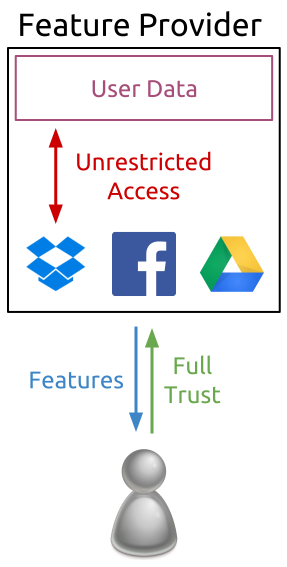
\includegraphics[height=2in]{./figs/out/TrustModel-Traditional.pdf}
    \caption{Traditional Trust Relationships}
    \label{fig:mitigation:trust:traditional}
  \end{subfigure}
  ~
  \begin{subfigure}[t]{0.48\textwidth}
    \centering
    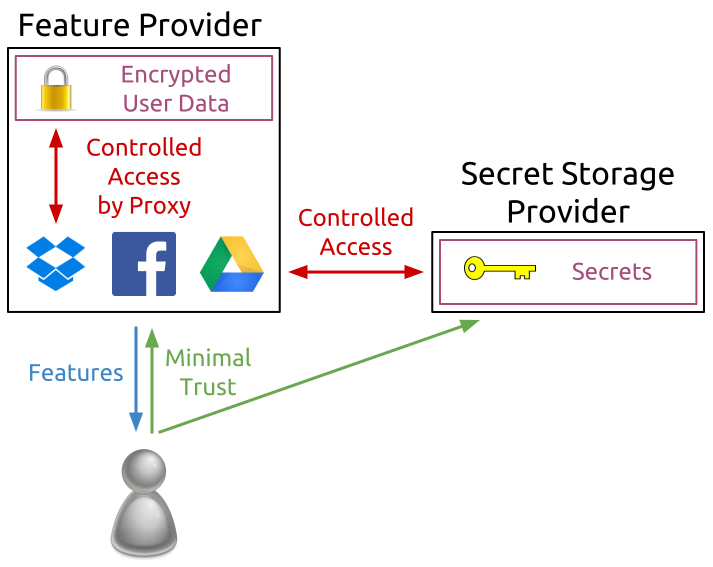
\includegraphics[height=2in]{./figs/out/TrustModel-Seperated.pdf}
    \caption{Distributed Trust Relationship}
    \label{fig:mitigation:trust:distributed}
  \end{subfigure}
  \caption{Trust Relationships}
  \label{fig:mitigation:trust}
\end{figure}

Techniques such as these are a from of ``trust distribution'' --
e.g. a technique for reducing trust in individual third parties by
instead spreading it across multiple parties
(Figure~\ref{fig:mitigation:trust}). Similar techniques have been used
within cryptographic protocols for the purpose of eliminating
single-points-of-trust~\cite{shamir1979}.\footnote{Such techniques
  also bear some resemble to previously proposed ``escrow systems,
  albeit with a somewhat opposite end-goal~\cite{denning1996}.} Such
techniques are capable of allowing users reduce or eliminate trust
surpluses across a range of use cases without introducing significant
additional usage burdens. While there are approaches to limiting third
party trust that aim to avoid trusting any third party (e.g. the OTR
chat protocol~\cite{otr-v3}), such techniques are often difficult to
apply generally or to use without imposing additional usability
burdens on end users. Trust distribution, however, provides a
relatively generic approach to to eliminating trust in any single
third party (or when coupled with techniques such
as~\cite{shamir1979}, even larger subsets of all involved parties).

To summarize, the basic practice of reducing the number of trusted
capabilities afforded to third parties is as follows: first, identity
any surplus trusted capabilities, next leverage cryptographic
techniques to limit third party access to these capabilities, finally,
leverage techniques such as SSaaS to store and control access to any
secret materials required by the aforementioned cryptographic
techniques in a manner that avoids burdening the end user with the
need to manage such secrets manually. This process eliminates trust
surplus and distributes user trust across multiple third parties in a
manner such that individual third parties can not subvert this
trust. As mentioned in \S~\ref{sec:analysis:violations}, such
arrangements do have the potential to encourage collusion-type trust
violations where multiple third parties work together to regain
capabilities that have bean denied to them. Mechanisms for
disincentivizing such violations will be discussed in the next
section.

\subsection{Disincentivizing Violations}
\label{sec:mitigation:violations}

Beyond limiting number of capabilities users must entrust to third
parties, it is also desirable to disincentive the mechanism by which
third parties might violate such trust.  While technological solution
provide options for reducing degree of trust, it is largely policy
solution that will drive the disincentivization of common classes of
trust violations. By disincentivizing certain classes of trust
violations, we can reduce the likelihood that third parties will
commit such violations, leading to more ``trustworthy'' third parties
and fewer instances of trust violations. There are a variety of
mechanism that one might employ with an aim toward disincentivizing
trust violations. I discusses several of the more prominent ones in
this section.

\subsubsection{Distributed Trust Markets}

In today's single-trust relationships, users primarily select third
party services on the basis of their features. When users pay for
these services, they're primarily paying to support the core features
such services provide. Privacy and security, while potential concerns,
are at best secondary goals. Furthermore, on many free cloud services,
the ability to harvest user data is the basis of the service
provider's business model. As discussed in
Section~\ref{sec:mitigation:capabilites}, these situations create a
number of perverse incentives in terms of a third party's respect to
user security and privacy. In the first case, the third party simply
does not prioritize user security since that is not the primary basis
on which users are choosing to pay for a service. In the second case,
a third party service provider actively works to subvert user security
and privacy in order to further leverage user data to generate income.

Distributed trust relationships such as those provided by the SSaaS
architecture aim to rectify these issues by introducing additional
third party actors whose primary goal is the protection of user
secrets and from whom users purchase secret storage services on the
basis of security and privacy guarantees. The ability of distributed
trust architectures to separate secret storage duties from feature
provider duties allows users to purchase each service on the basis of
its associated merits, avoiding the issues associated with putting
features in direct competition with security and privacy -- a
competition that security and privacy have historically lost. Thus,
distributed trust relationships not only allow users to eliminate
trust surpluses, they also allow users to escape from the artificial
trade off between desirable feature sets and the control and privacy
of their data. Given such separation, independent markets can form
around feature provision and secret protection, optimized for the
respective priorities of each field.

Beyond the removal of perverse incentives brought about by the
distribution of trust across multiple parties, it is also desirable to
encourage a competitive market amongst multiple secret storage
providers. In order to achieve such a market, it is necessary to
standardize a single multi-party-compatible distributed trust
protocol. Such a standard protocol gives users a high degree of
mobility between competing secret storage providers, avoiding vendor
lock-in. This mobility, in turn, increases the competitive pressures
between providers. In short, the aim of a distributed trust ecosystem
is to make security and privacy tradable commodities, and to leverage
market powers to price and improve both. A competitive market for
secret storage has a number of security and privacy enhancing
benefits:

\begin{packed_desc}
\item[Reputation:] If users can easily switch between secret storage
  providers, it forces such providers to compete on the basis of their
  security and privacy preserving reputations. Providers who can do a
  superior job avoiding the trust violations discussed in
  \S~\ref{sec:analysis:violations} can attract more users and/or
  command a higher price for their services. Since a secret storage
  provider reputation is tied solely to their ability to faithfully
  protect user secrets, they will not be able to ``iron over'' any
  privacy-related reputation failings with superior end user feature
  sets -- a practice employed by many traditional feature
  providers.\footnote{As an example, consider Facebook's numerous
    trust violations~\cite{goel2014, lomas2014, tsukayama2014} and the
    fact that such violations have had no noticeable impact on the
    number of people using Facebook~\cite{foster2014}. An secret
    storage provider would enjoy no such network benefit from
    providing additional services beyond secret storage were they to
    violate user's trust; instead, users would simply switch to a new
    provider.}
\item[Multiple Providers:] A healthy ecosystem of competing secret
  storage providers will allow users to select from multiple
  independent providers over which they may further distribute their
  trust beyond a binary feature provider + secret storage provider
  relationship. Such sharding provides a number of benefits over
  relying on a single SSP, from additional trust reduction to data
  redundancy.
\item[Cost:] As in other competitive markets, having a number of
  competing providers will allow the user to select a provider that
  offers the best combination of cost and service.
\end{packed_desc}

Distributed trust markets are potentially useful at disincentivizing a range
of trust violations, from implicit violations to unintentional
violations. Such markets help to align economic incentives that
practices that disfavor such violations.

\subsubsection{Digital Due Process}

While mechanisms such as distributes trust markets are useful for
disincentivizing many classes of trust violations, other mechanisms
are needed to disincentive compelled violations. Trust markets
potentially encourage third parties to push back against compelled
trust violations to the maxim extent permitted under the law, but they
do little to protect users in cases where the law heavily favors
compelled trust violations even in cases where such violations are not
in the public interest. To reduce such violations, it is necessary to
protect ``digital due process'' rights.

The first step toward protecting such rights is to ensure that user
data stored or processed by third party services receives the same
level of protection as data stored or processed locally. This concept
runs counter to the Third Party Doctrine established bu current
U.S. case law~\cite{thompson-thirdparty}. This doctrine holds that
individuals who voluntarily store their data with third parties have
no ``reasonable expectation of privacy''~\cite{scotus-katzvus} for
such data. While such a viewpoint may have made sense in the mid
20\textsuperscript{th} century when it was established via a series of
Supreme Court rulings~\cite{scotus-usvmiller-privacy,
  scotus-smithvmaryland}, it does not translate well to a world where
third party access to user data is the norm. As shown in
\S~\ref{sec:analysis:violations} compelled violations are a growing
trend, and in many cases, such violations are served via third-party
doctrine mechanisms. Such trends suggest a likely overreach of
government data collection, leading to a range of potential adverse
effect (e.g.~\cite{penney2016}). One possible way of halting or
reversing this trend would be to eliminate the third party doctrine
and begin requiring a 4\textsuperscript{th} Amendment warrant in order
to compel third to provide or modify user data.

Fortunately, changes to the third party doctrine are beginning to
progress on multiple fronts. Recent Supreme Court decisions have
suggested a willingness to expand user privacy rights in the digital
realm, and may eventually lead the Supreme Court to revisit the third
party doctrine~\cite{scotus-usvjones}.  Congress has also long been
departing updates to third-party doctrine derived laws such a the
Electronic Communications Privacy Act (ECPA)~\cite{ecpa} to include a
warrant requirement for digitally stored
emails~\cite{eff-ecpareform}. Recently, the U.S. House of Represents
even unanimously passed a bill to amend the ECPA to required warrants
in most cases~\cite{trujillo-ecpa}. Such movements suggest a growing
recognition of the due process rights of digital data, regardless of
whether it is stored locally or by third parties. Such trends likely
represent the best hope for reducing unnecessary compelled violations,
ensuring such violations only occur in cases where the public interest
in significantly favored by the violation of user trust.

\subsubsection{Cyber Liability}

%%  LocalWords:  SSaaS SSP OTR FP th ECPA
